\documentclass[20pt,landscape,dvips]{foils} 
% add 'draft' option above to exclude image when compiling
\usepackage[french]{babel}
\usepackage[utf8]{inputenc}  
\usepackage[french=guillemets*]{csquotes} 
\MakeOuterQuote{"}
\frenchspacing
\DecimalMathComma

\usepackage{latexsym}
\usepackage{amsmath,amssymb,amsfonts}
\usepackage{MnSymbol}
\usepackage{url}
\usepackage{graphicx}
%\usepackage[dvipsnames]{xcolor}
\usepackage{hyperref}
\usepackage{alltt}
\usepackage{pifont,manfnt}
\usepackage[dvipsnames,table]{xcolor}
\usepackage{subfig}
%\usepackage{enumerate}
%\usepackage{colortbl}
\usepackage{multirow,hhline}
\usepackage{cclicenses}
\setlength\parindent{0pt}
\hypersetup{colorlinks=true,citecolor=black,urlcolor=black,linkcolor=black}
\usepackage[style=verbose]{biblatex}
\bibliography{refs}

\newcommand{\highlight}[1]{\textcolor{Plum}{\bfseries #1}}
\newcommand{\remark}[1]{%
%\centerline{
\begin{center}
\framebox[.9\textwidth][t]{
\ding{46} 
\parbox[t]{.8\textwidth}{\small #1}}
\end{center}}

\DeclareMathOperator*{\inlaw}{\sim}
\newcommand{\iid}{\inlaw_{\text{i.i.d.}}}
%\newcommand{\iid}{\mathop{\mathrm{diag}}}
\newcommand{\pobs}{p_{\text{obs}}}

\reversemarginpar
\def\mark{\marginpar{\dbend}}

%\newcommand{\bm}[1]{\mbox{\boldmath{$#1$}}}
\renewcommand{\abstractname}{Summary}
\newcommand\bs{\char '134}   %  a backslash character for the \tt font
%\renewcommand\refname{Additional Readings}

% customize header/footer
\rightheader{}
% Note about the copyleft symbol:
% I use a custom reversed and circled "c" char because \textcopyleft in
% the textcomp package does not support sans serif font.
% Also, "c" is shifted horizontally by 1ex to align with the circle.
%\Restriction{\mbox{\raisebox{1.5ex}{\rotatebox{180}{\textcircled{c\kern.1ex}}} 2009}, \url{www.aliquote.org}}
% now I use the CC licence...
% \Restriction{\cc 2016 \VCRevision}
\Restriction{\cc 2016 Module 11 EESPE}

\title{Méthodes psychométriques en qualité de vie}
\author{Christophe Lalanne\\EA 7334 REMES\\ Unité de Méthodologie des critères d’évaluation\\Université Paris-Diderot, Sorbonne Paris-Cité\\}
\date{
\includegraphics[height=18ex]{logo.eps}}

%%% This file has been generated by the vc bundle for TeX.
%%% Do not edit this file!
%%%
%%% Define Git specific macros.
\gdef\GITHash{f4328f7906d309e9224e3e5c2f7f36477f44e69f}%
\gdef\GITAbrHash{f4328f7}%
\gdef\GITParentHashes{136657e4877819e72dc9ebb2f209631a2a8d1057}%
\gdef\GITAbrParentHashes{136657e}%
\gdef\GITAuthorName{Christophe Lalanne}%
\gdef\GITAuthorEmail{ch.lalanne@gmail.com}%
\gdef\GITAuthorDate{2016-07-06 10:29:58 +0200}%
\gdef\GITCommitterName{Christophe Lalanne}%
\gdef\GITCommitterEmail{ch.lalanne@gmail.com}%
\gdef\GITCommitterDate{2016-07-06 10:29:58 +0200}%
%%% Define generic version control macros.
\gdef\VCRevision{\GITAbrHash}%
\gdef\VCAuthor{\GITAuthorName}%
\gdef\VCDateRAW{2016-07-06}%
\gdef\VCDateISO{2016-07-06}%
\gdef\VCDateTEX{2016/07/06}%
\gdef\VCTime{10:29:58 +0200}%
\gdef\VCModifiedText{\textcolor{red}{with local modifications!}}%
%%% Assume clean working copy.
\gdef\VCModified{0}%
\gdef\VCRevisionMod{\VCRevision}%


\begin{document}
\LogoOff
\maketitle
\rightfooter{\quad\textsf{\thepage}}



%---------------------------------------------------------------Slide-
\foilhead{Analyses factorielles : extensions}
\begin{itemize}
\item Indices de modification
\item Approche multi-groupes
\item Invariance de mesure
\item Cas des données catégorielles
\end{itemize}



%---------------------------------------------------------------Slide-
\foilhead{Modèle de mesure et modèle structurel}

{\centering 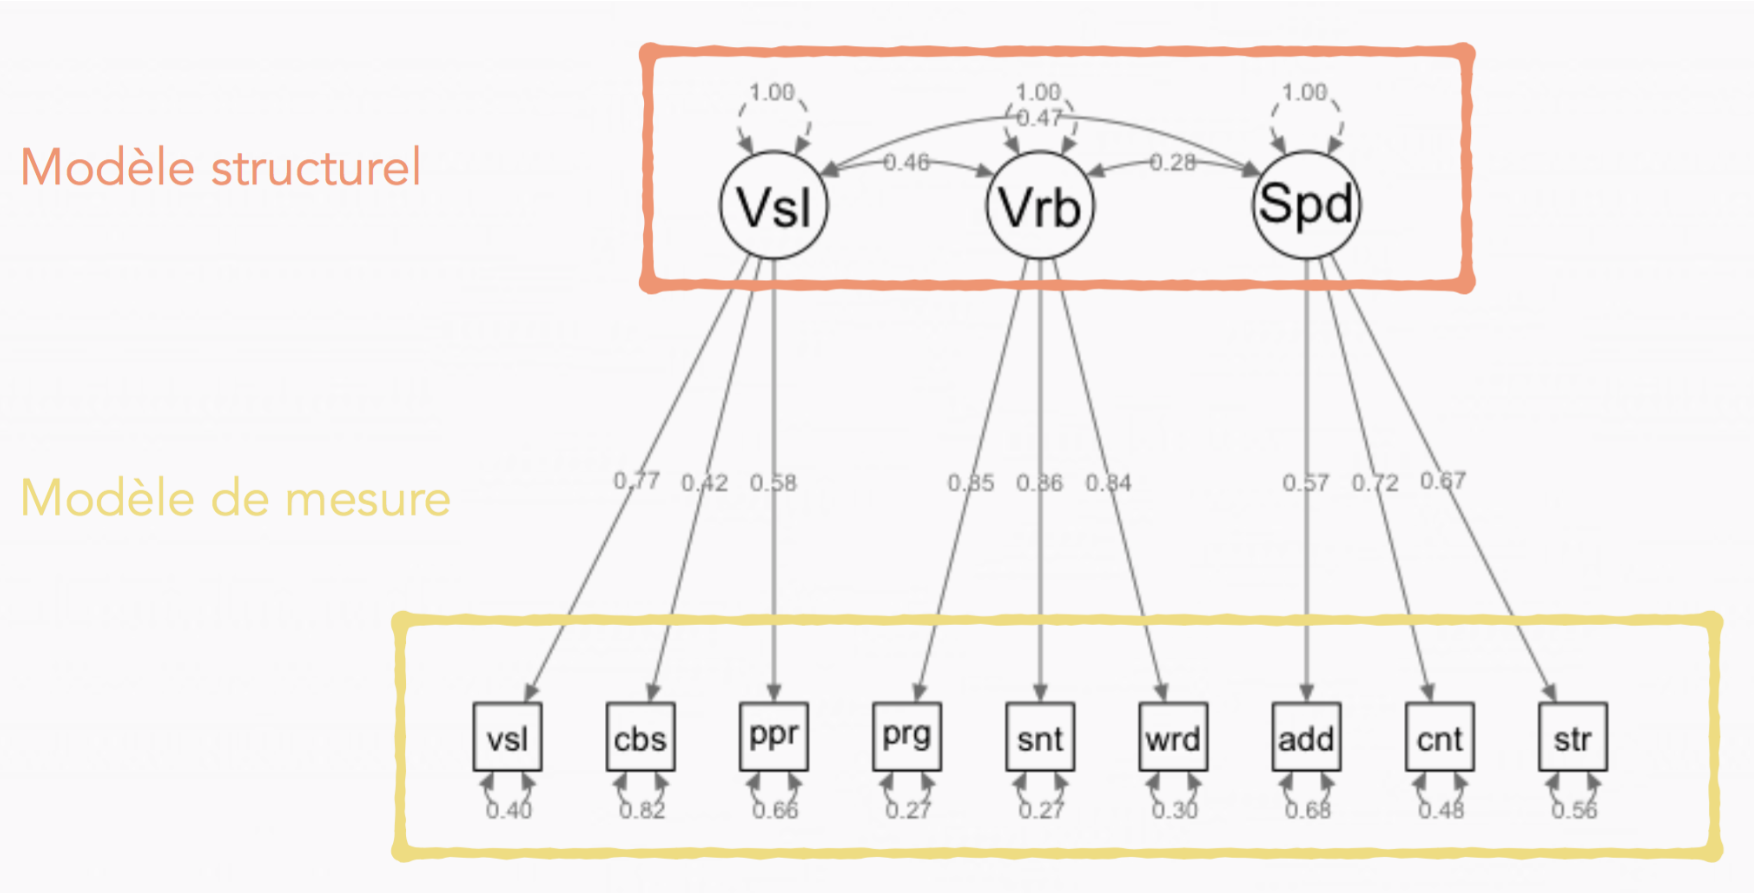
\includegraphics[width=.85\textwidth]{figs/HS3.eps}\par}

%---------------------------------------------------------------Slide-
\foilhead{Identification du modèle}

{\centering 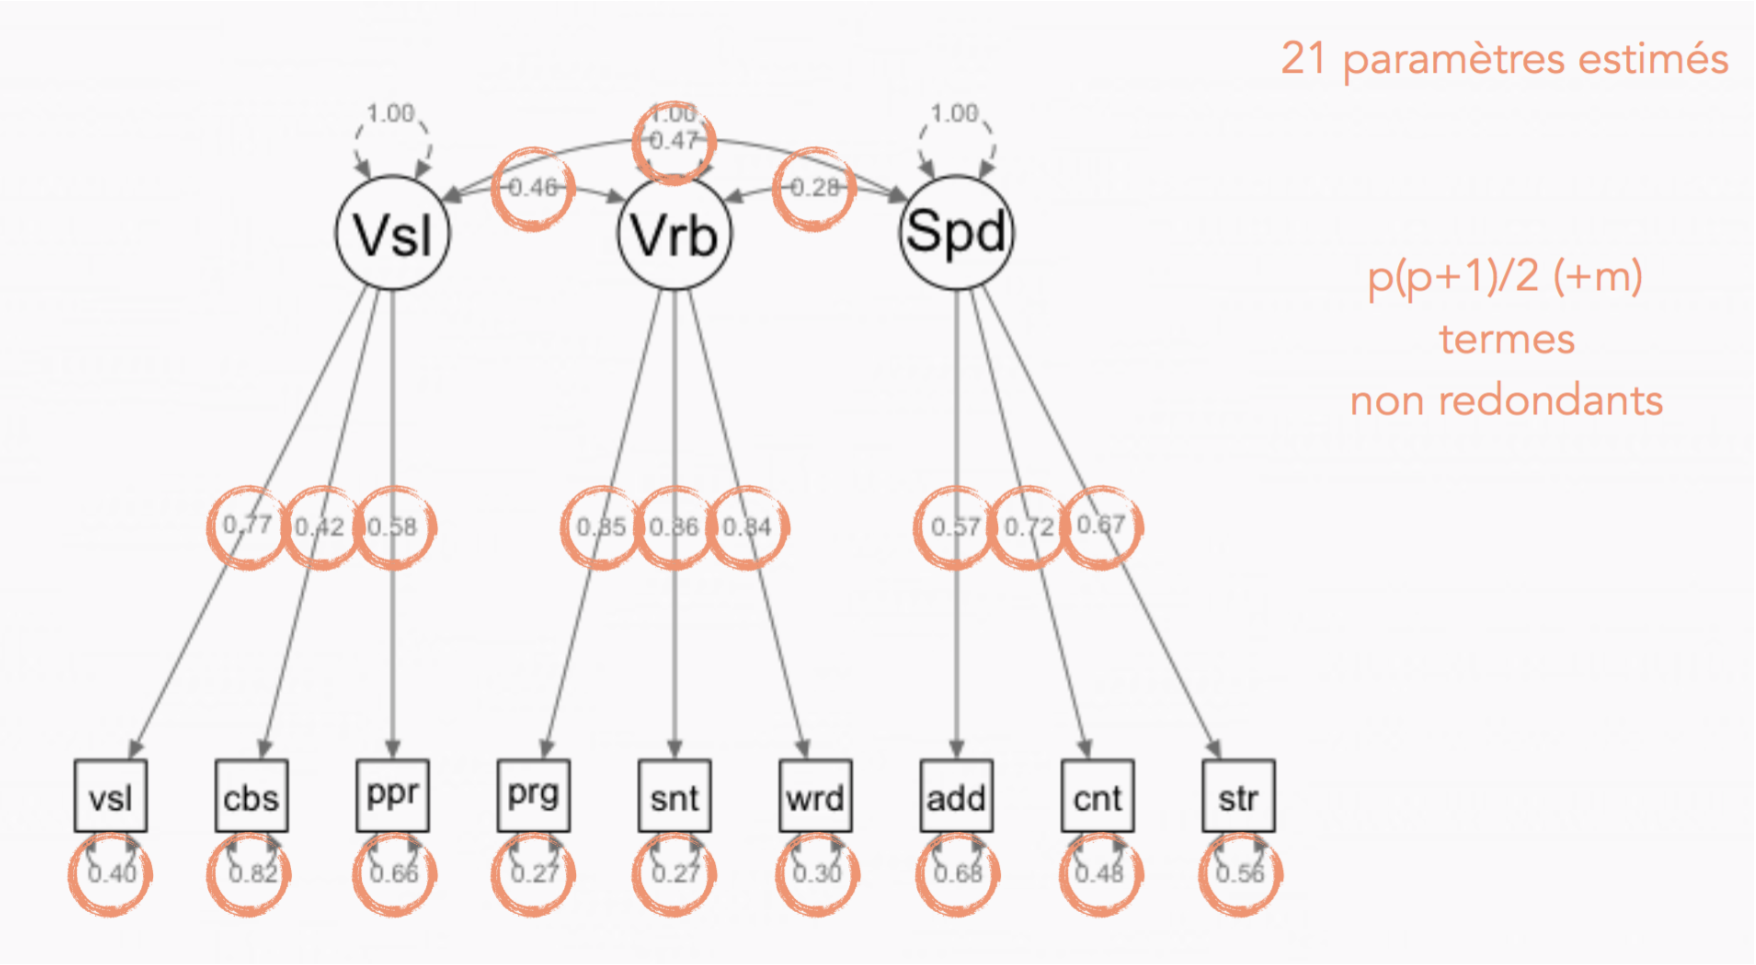
\includegraphics[width=.85\textwidth]{figs/cfa3.eps}\par}

%---------------------------------------------------------------Slide-
\foilhead{Interprétation des coefficients}

{\centering 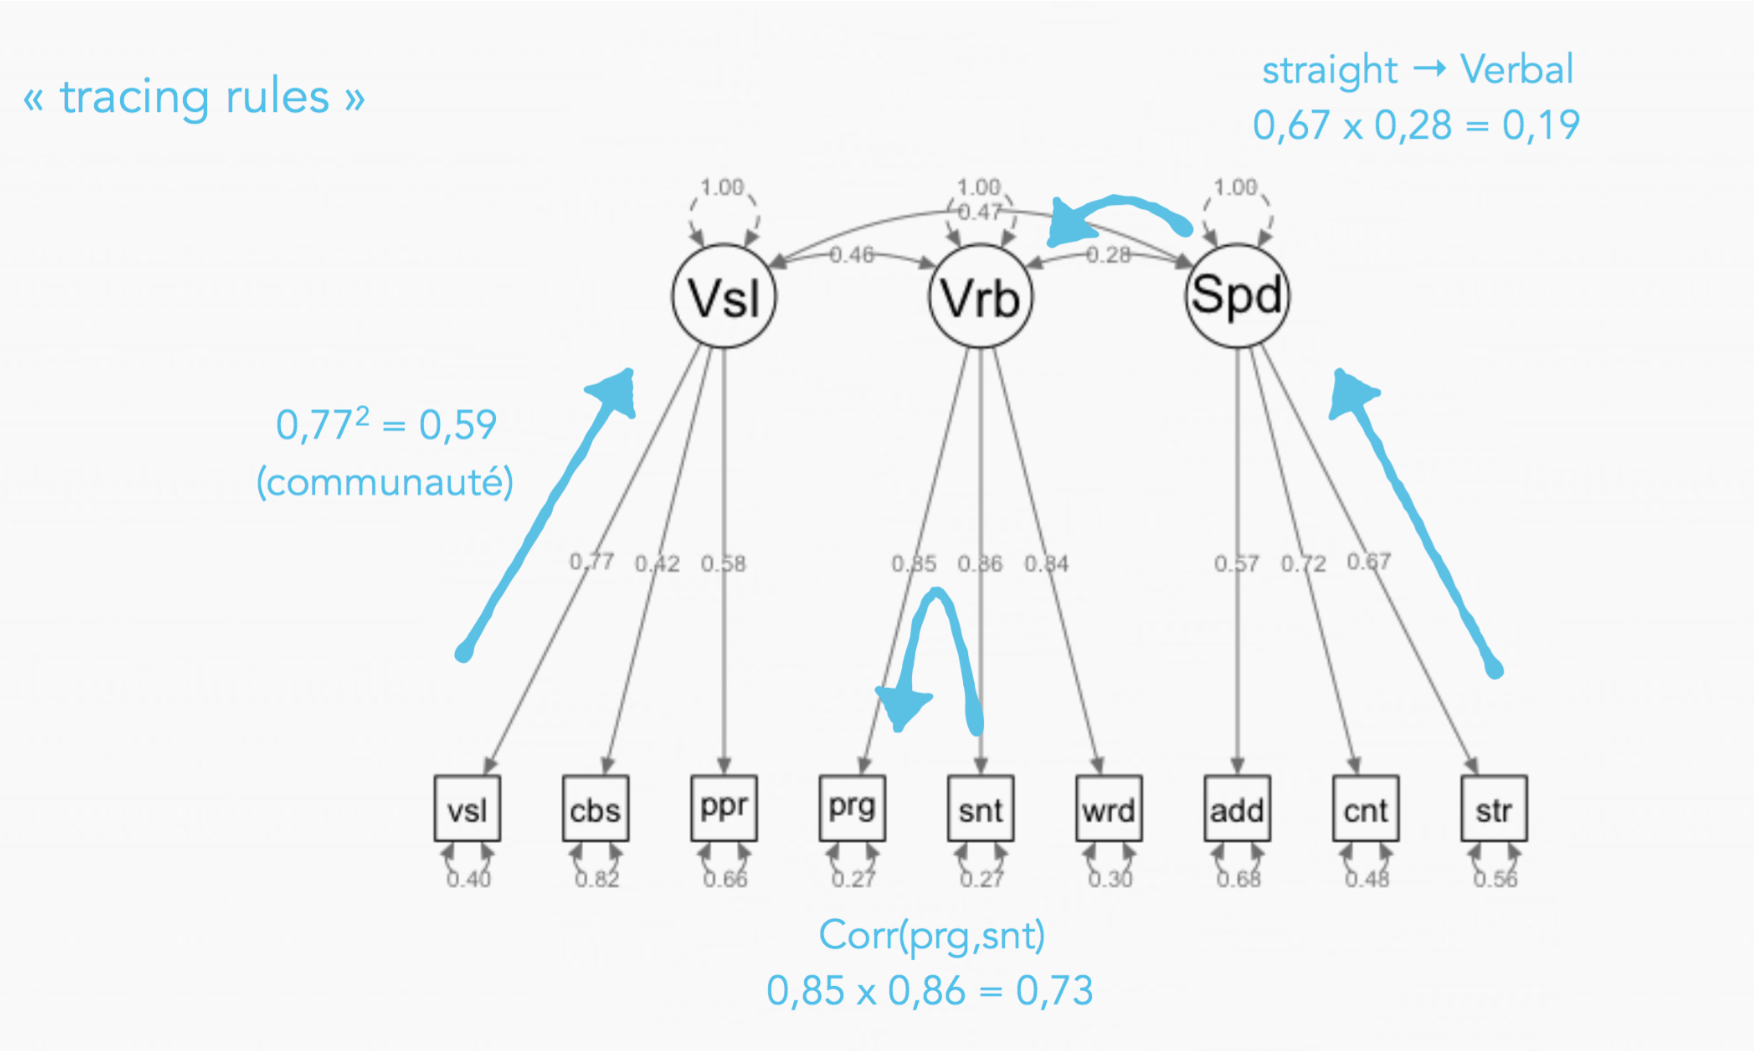
\includegraphics[width=.85\textwidth]{figs/cfa2.eps}\par}


%---------------------------------------------------------------Slide-
\foilhead{Syntaxe \texttt{lavaan}}
Notre modèle réflexif de base (3 facteurs corrélés) s'écrit :
\begin{alltt}
m <- 'Visual =~ visual + cubes + paper 
      Verbal =~ paragrap + sentence + wordm
      Speed  =~ addition + counting + straight'
\end{alltt}

\begin{itemize}
\item \verb|=~| régression MV - LV 
\item \verb|~~| covariance LV-LV, corrélation MV - MV 
\item \verb|~| régression LV-LV 
\item \texttt{==} contraintes (identification ou autre) 
\item \texttt{:=} construction d’un nouveau terme de modèle
\end{itemize}


%---------------------------------------------------------------Slide-
\foilhead{Modèles de covariance}
L'avantage des modèles CFA est de permettre de quantifier l'écart entre le
modèle et les données, de tester si cet écart est significativement différent de
ce qu'on attendrait sous $H_0$, et de comparer des modèles emboîtés.

\begin{alltt}
C <- cov(d)
N <- nrow(d)
r <- cfa(m, std.lv = TRUE, sample.cov = cov(d), sample.nobs = N)
resid(r)
\end{alltt}

La matrice\mark{} de covariance utilisée par \texttt{lavaan} est calculée avec
  un dénominateur à $N$ et non $N-1$ (méthode ML).


%---------------------------------------------------------------Slide-
\foilhead{Indices de modification}
Il est parfois nécessaire de vérifier s'il n'exsiste pas des déviations locales
au modèle postulé (en particulier au niveau des résidus), en particulier ajouter
des paramètres susceptibles d'améliorer la qualité globale d'ajustement du
modèle\autocite{brown06}.
\begin{alltt}
r <- cfa(m, data = d)
standardizedSolution(r)
resid(r)       \ding{182}
modindices(r)  \ding{183}
\end{alltt}


%---------------------------------------------------------------Slide-
\foilhead{}

\begin{alltt}
m1 <- 'Visual =~ visual + cubes + paper 
       Verbal =~ paragrap + sentence + wordm
       Speed  =~ addition + counting + straight'

m2 <- 'Visual =~ visual + cubes + paper 
       Verbal =~ paragrap + sentence + wordm
       Speed  =~ addition + counting + straight
       addition ~~ counting'  \ding{182}
r1 <- cfa(m1, data = d)
r2 <- cfa(m2, data = d)
anova(r1, r2)                 \ding{183}
\end{alltt}


%---------------------------------------------------------------Slide-
\foilhead{Analyse stratifiée sur plusieurs groupes}
\highlight{Première approche :} estimer séparément les modèles dans les deux groupes définis
par la variable \texttt{school}.

\begin{alltt}
r3 <- cfa(m1, data = HS, group = "school")
r3
\end{alltt}

\highlight{Deuxième approche :} contraindre les charges factorielles à être
égales dans les deux groupes.

\begin{alltt}
r4 <- cfa(m1, data = HS, group = "school", 
          group.equal = "loadings")
r4
\end{alltt}


% ---------------------------------------------------------------Slide-
\foilhead{Invariance de mesure}
Pour garantir des comparaisons de groupes valides, il faut au préalable
s'assurer que l'on mesure bien la même chose de la même manière\autocite{teresi06}. 
\begin{enumerate}
\item \textcolor{CornflowerBlue}{Invariance configurale} : structure factorielle identique entre groupes
\item \textcolor{CornflowerBlue}{Invariance faible} : égalité des charges factorielles entre groupes
\item \textcolor{CornflowerBlue}{Invariance forte} : égalité des moyennes entre groupes
\item \textcolor{CornflowerBlue}{Invariance stricte} : égalité des erreurs entre groupes
\item Invariance stricte + égalité des variances LV ; Invariance stricte +
  égalité des variances LV + égalité des moyennes LV ; Invariance partielle :
  conditions non vérifiées pour l'ensemble des MV 
\end{enumerate}

% ---------------------------------------------------------------Slide-
\foilhead{Invariance et comparaison de groupes\autocite{beaujean14}}

{\centering 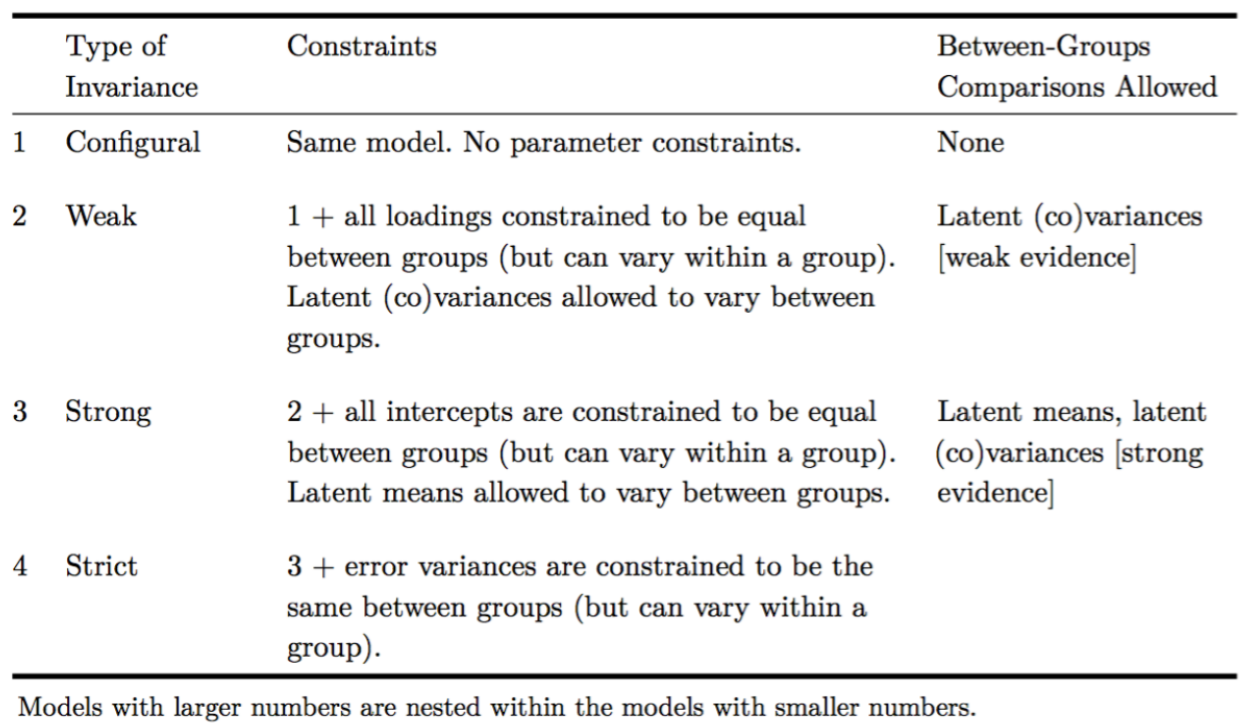
\includegraphics[width=.7\textwidth]{figs/ivmeas.eps}\par}


% ---------------------------------------------------------------Slide-
\foilhead{Le package \texttt{semTools}}

{\centering 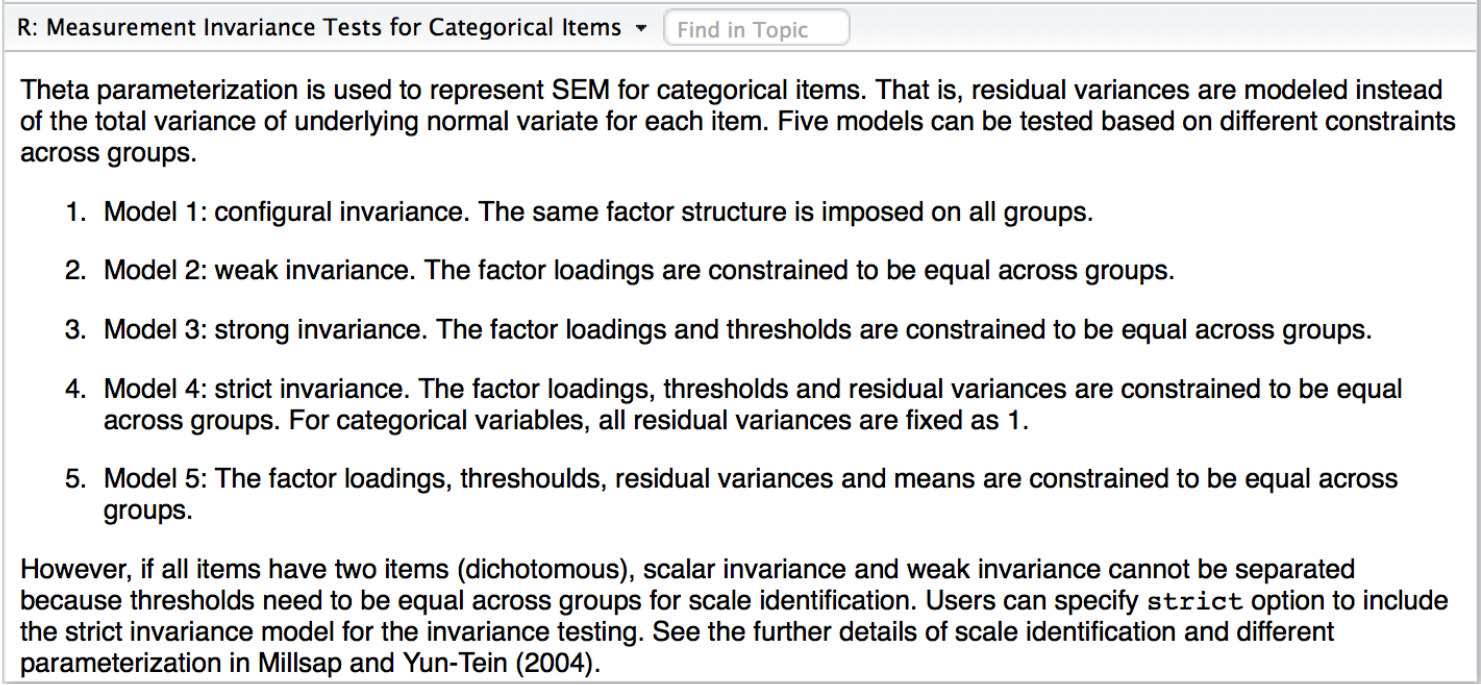
\includegraphics[width=.7\textwidth]{figs/semTools.eps}\par}


% ---------------------------------------------------------------Slide-
\foilhead{Illustration}

\begin{alltt}
library(semTools)
measurementInvariance(model = m, data = d, 
                      group = "school") \hfill \ding{182}
measurementInvariance(model = m, data = d, 
                      group = "school", \highlight{strict = TRUE}) \hfill \ding{183}
\end{alltt}

La comparaison des modèles emboîtés 1 à 4 (\texttt{\ding{182}}) est suffisante
quand on s'intéresse au modèle de mesure et à la comparaison de scores d'un
questionnaire.

% ---------------------------------------------------------------Slide-
\foilhead{Dimensions \emph{versus} catégories}
L'analyse factorielle suppose que les variables manifestes et latentes sont
continues. En pratique, en psychiatrie ou en qualité de vie, les mesures
auto-rapportées reposent sur des items dichotomiques (oui/non) ou polytomiques
(type Likert).

Cas des données catégorielles : modèle de type IRT ou FA sur matrice de
corrélation appropriée (IFA, package \texttt{psych}), choix d'un estimateur
approprié (WLSM(V)/DWLS et paramétrisation theta\autocite{muthen93}).

Le package \texttt{lavaan} permet de traiter le cas des variables catégorielles
et fournit des modèles à seuil\autocite[chap.~6]{beaujean14}.

% ---------------------------------------------------------------Slide-
\foilhead{Exemple\autocite{partchev04}}

Quelle est la surface d'un cercle ayant un rayon de 3 cm ?
\begin{description}
\item[(a)] $9,00$ cm$^2$
\item[(b)] $18,85$ cm$^2$
\item[(c)] $28,27$ cm$^2$  
\end{description}

% ---------------------------------------------------------------Slide-
\foilhead{}

{\centering 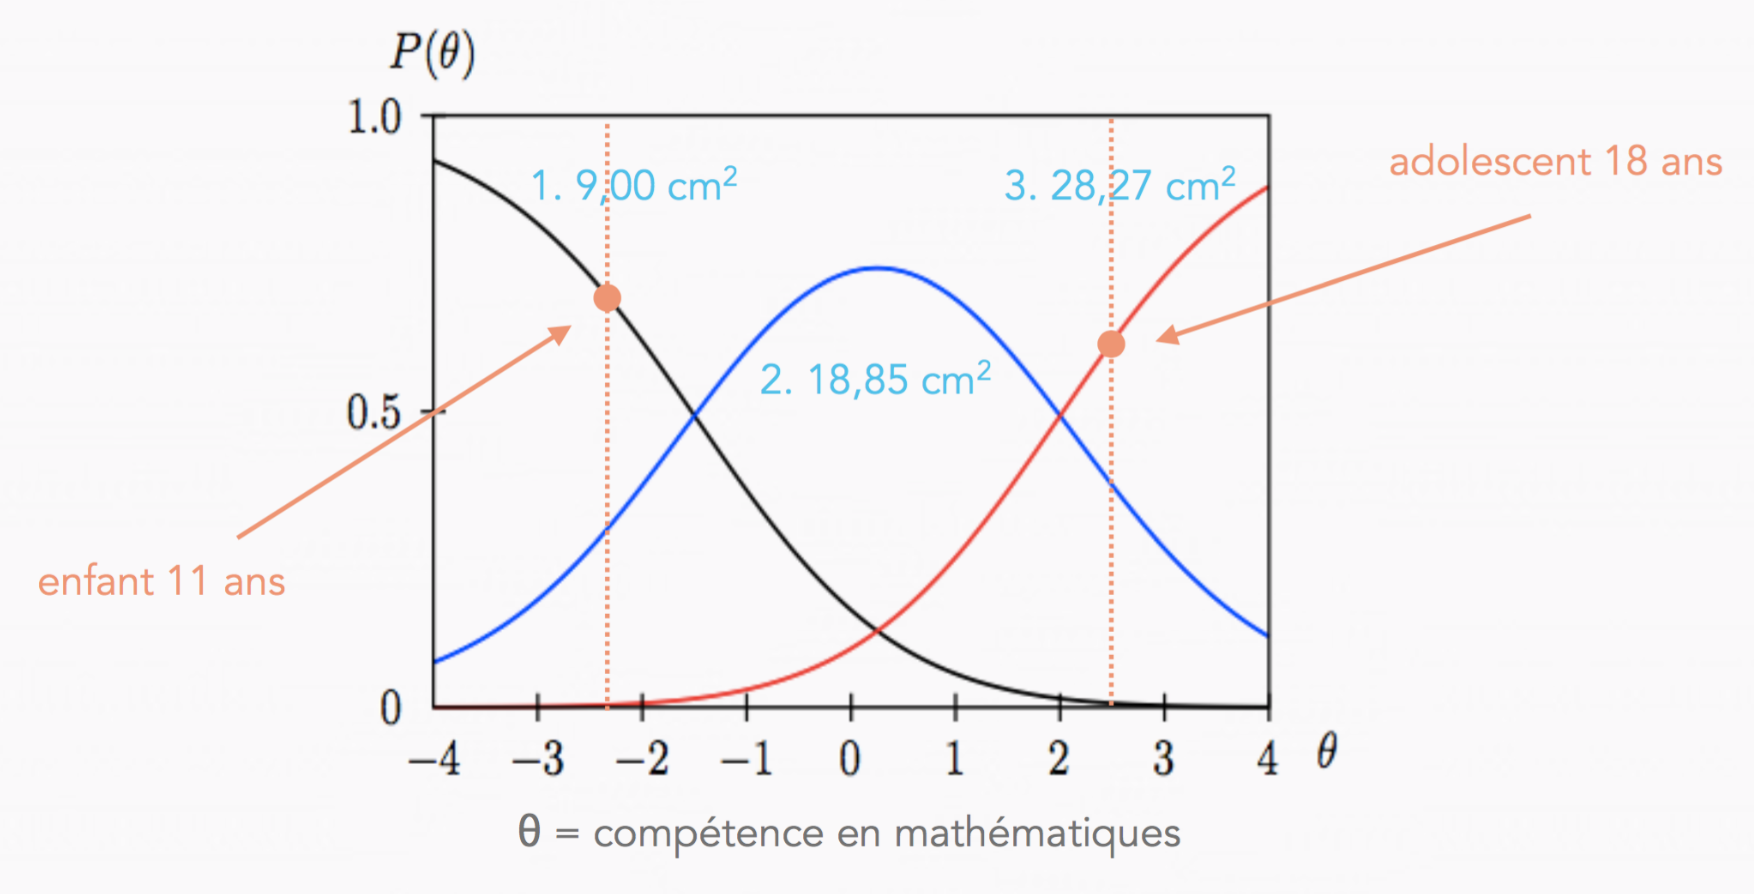
\includegraphics[width=.85\textwidth]{figs/math.eps}\par}


% ---------------------------------------------------------------Slide-
\foilhead{Estimateurs WLS}

{\centering \includegraphics[width=.7\textwidth]{figs/wls.eps}\par}


% ---------------------------------------------------------------Slide-
\foilhead{Illustration : ACP sur matrice de corrélation polychorique} 

Echelle HADS à 2 dimensions ($N=201$ patients) :
\begin{alltt}
load("HADS.RData")
dep <- c(1,3,4,5,9,13,14)
anx <- seq(1,14)[-c(1,3,4,5,9,13,14)]
library(polycor)
ddep <- as.data.frame(lapply(data[,dep], as.ordered)) \hfill \ding{182}
C <- hetcor(ddep) \hfill \ding{183}
principal(C$correlations, rotate = "none")
\end{alltt}

% ---------------------------------------------------------------Slide-
\foilhead{Illustration : CFA sur données catégorielles}
\highlight{Deux options :} travailler avec la matrice de corrélations
polychoriques ou utiliser les fonctionnalités de \texttt{lavaan}.

Premier cas de figure :
\begin{alltt}
m <- 'Dep ~ Y1 + Y3 + Y4 + Y5 + Y9 + Y13 + Y14'
r <- cfa(model = m, sample.cov = C$correlations, 
         sample.nobs = nrow(ddep), std.lv = TRUE)
parameterEstimates(r, ci = FALSE, standardized = TRUE)
\end{alltt}

Deuxième cas de figure (suppose que les variables sont des facteurs avec
des niveaux ordonnés) :
\begin{alltt}
r <- cfa(model = m, data = ddep, std.lv = TRUE)
\end{alltt}

% ---------------------------------------------------------------Slide-
\foilhead{}

Fichier de données et scripts R disponibles à l'adresse suivante :\newline
{\centering \url{https://bitbucket.org/chlalanne/eespe11}\par}
\vfill

\raggedleft \scriptsize -- Typeset with \FoilTeX\ (version 2), Revision \VCRevision

\end{document}
